\XtoCBlock{Sum}
\label{block:Sum}
\begin{figure}[H]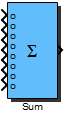
\includegraphics{Sum}\end{figure} 

\begin{XtoCtabular}{Inports}
In1 & Input \#1\tabularnewline
\hline
In2 & Input \#2\tabularnewline
\hline
In3 & Input \#3\tabularnewline
\hline
In4 & Input \#4\tabularnewline
\hline
In5 & Input \#5\tabularnewline
\hline
In6 & Input \#6\tabularnewline
\hline
In7 & Input \#7\tabularnewline
\hline
In8 & Input \#8\tabularnewline
\hline
\end{XtoCtabular}


\begin{XtoCtabular}{Outports}
Out & Result\tabularnewline
\hline
\end{XtoCtabular}

\begin{XtoCtabular}{Mask Parameters}
In1 & Input \#1\tabularnewline
\hline
In2 & Input \#2\tabularnewline
\hline
In3 & Input \#3\tabularnewline
\hline
In4 & Input \#4\tabularnewline
\hline
In5 & Input \#5\tabularnewline
\hline
In6 & Input \#6\tabularnewline
\hline
In7 & Input \#7\tabularnewline
\hline
In8 & Input \#8\tabularnewline
\hline
\end{XtoCtabular}

\subsubsection*{Description:}
Sum of inputs:

    + ... Input will be added to result.

    - ... Input will be subtracted from result.

    0 ... Input will be ignored.

\subsubsection*{Implementations:}
\begin{tabular}{l l}
\textbf{FiP8} & 8 Bit Fixed Point Implementation\tabularnewline
\textbf{FiP16} & 16 Bit Fixed Point Implementation\tabularnewline
\textbf{FiP32} & 32 Bit Fixed Point Implementation\tabularnewline
\textbf{Float32} & 32 Bit Floating Point Implementation\tabularnewline
\textbf{Float64} & 64 Bit Floating Point Implementation\tabularnewline
\end{tabular}

\XtoCImplementation{FiP8}
\index{Block ID!4800}
\nopagebreak[0]
% Implementation details
\begin{tabular}{l l}
\textbf{Name} & FiP8 \tabularnewline
\textbf{ID} & 4800 \tabularnewline
\textbf{Revision} & 0.1 \tabularnewline
\textbf{C filename} & Sum\_FiP8.c \tabularnewline
\textbf{H filename} & Sum\_FiP8.h \tabularnewline
\end{tabular}
\vspace{1ex}

8 Bit Fixed Point Implementation

\begin{XtoCtabular}{Controller Parameters}
sign & Bitfield with sign information of inputs\tabularnewline
\hline
\end{XtoCtabular}

% Implementation data structure
\XtoCDataStruct{Data Structure:}
\begin{lstlisting}
typedef struct {
     uint16        ID;
     int8          *In1;
     int8          *In2;
     int8          *In3;
     int8          *In4;
     int8          *In5;
     int8          *In6;
     int8          *In7;
     int8          *In8;
     int8          Out;
     uint16        sign;
} SUM_FIP8;
\end{lstlisting}

\ifdefined \AddTestReports
\InputIfFileExists{\XcHomePath/Library/Math/Doc/Test_Sum_FiP8.tex}{}{}
\fi
\XtoCImplementation{FiP16}
\index{Block ID!4801}
\nopagebreak[0]
% Implementation details
\begin{tabular}{l l}
\textbf{Name} & FiP16 \tabularnewline
\textbf{ID} & 4801 \tabularnewline
\textbf{Revision} & 0.1 \tabularnewline
\textbf{C filename} & Sum\_FiP16.c \tabularnewline
\textbf{H filename} & Sum\_FiP16.h \tabularnewline
\end{tabular}
\vspace{1ex}

16 Bit Fixed Point Implementation

\begin{XtoCtabular}{Controller Parameters}
sign & Bitfield with sign information of inputs\tabularnewline
\hline
\end{XtoCtabular}

% Implementation data structure
\XtoCDataStruct{Data Structure:}
\begin{lstlisting}
typedef struct {
     uint16        ID;
     int16         *In1;
     int16         *In2;
     int16         *In3;
     int16         *In4;
     int16         *In5;
     int16         *In6;
     int16         *In7;
     int16         *In8;
     int16         Out;
     uint16        sign;
} SUM_FIP16;
\end{lstlisting}

\ifdefined \AddTestReports
\InputIfFileExists{\XcHomePath/Library/Math/Doc/Test_Sum_FiP16.tex}{}{}
\fi
\XtoCImplementation{FiP32}
\index{Block ID!4802}
\nopagebreak[0]
% Implementation details
\begin{tabular}{l l}
\textbf{Name} & FiP32 \tabularnewline
\textbf{ID} & 4802 \tabularnewline
\textbf{Revision} & 0.1 \tabularnewline
\textbf{C filename} & Sum\_FiP32.c \tabularnewline
\textbf{H filename} & Sum\_FiP32.h \tabularnewline
\end{tabular}
\vspace{1ex}

32 Bit Fixed Point Implementation

\begin{XtoCtabular}{Controller Parameters}
sign & Bitfield with sign information of inputs\tabularnewline
\hline
\end{XtoCtabular}

% Implementation data structure
\XtoCDataStruct{Data Structure:}
\begin{lstlisting}
typedef struct {
     uint16        ID;
     int32         *In1;
     int32         *In2;
     int32         *In3;
     int32         *In4;
     int32         *In5;
     int32         *In6;
     int32         *In7;
     int32         *In8;
     int32         Out;
     uint16        sign;
} SUM_FIP32;
\end{lstlisting}

\ifdefined \AddTestReports
\InputIfFileExists{\XcHomePath/Library/Math/Doc/Test_Sum_FiP32.tex}{}{}
\fi
\XtoCImplementation{Float32}
\index{Block ID!4803}
\nopagebreak[0]
% Implementation details
\begin{tabular}{l l}
\textbf{Name} & Float32 \tabularnewline
\textbf{ID} & 4803 \tabularnewline
\textbf{Revision} & 0.1 \tabularnewline
\textbf{C filename} & Sum\_Float32.c \tabularnewline
\textbf{H filename} & Sum\_Float32.h \tabularnewline
\end{tabular}
\vspace{1ex}

32 Bit Floating Point Implementation

\begin{XtoCtabular}{Controller Parameters}
sign & Bitfield with sign information of inputs\tabularnewline
\hline
\end{XtoCtabular}

% Implementation data structure
\XtoCDataStruct{Data Structure:}
\begin{lstlisting}
typedef struct {
     uint16        ID;
     float32       *In1;
     float32       *In2;
     float32       *In3;
     float32       *In4;
     float32       *In5;
     float32       *In6;
     float32       *In7;
     float32       *In8;
     float32       Out;
     uint16        sign;
} SUM_FLOAT32;
\end{lstlisting}

\ifdefined \AddTestReports
\InputIfFileExists{\XcHomePath/Library/Math/Doc/Test_Sum_Float32.tex}{}{}
\fi
\XtoCImplementation{Float64}
\index{Block ID!4804}
\nopagebreak[0]
% Implementation details
\begin{tabular}{l l}
\textbf{Name} & Float64 \tabularnewline
\textbf{ID} & 4804 \tabularnewline
\textbf{Revision} & 0.1 \tabularnewline
\textbf{C filename} & Sum\_Float64.c \tabularnewline
\textbf{H filename} & Sum\_Float64.h \tabularnewline
\end{tabular}
\vspace{1ex}

64 Bit Floating Point Implementation

\begin{XtoCtabular}{Controller Parameters}
sign & Bitfield with sign information of inputs\tabularnewline
\hline
\end{XtoCtabular}

% Implementation data structure
\XtoCDataStruct{Data Structure:}
\begin{lstlisting}
typedef struct {
     uint16        ID;
     float64       *In1;
     float64       *In2;
     float64       *In3;
     float64       *In4;
     float64       *In5;
     float64       *In6;
     float64       *In7;
     float64       *In8;
     float64       Out;
     uint16        sign;
} SUM_FLOAT64;
\end{lstlisting}

\ifdefined \AddTestReports
\InputIfFileExists{\XcHomePath/Library/Math/Doc/Test_Sum_Float64.tex}{}{}
\fi
